%TODO kohrenz->resolution? wird nicht verwendet in auswertung


\documentclass[a4paper]{scrartcl}

\usepackage[utf8]{inputenc}
\usepackage[english]{babel}
\usepackage{lmodern} 
\usepackage[T1]{fontenc}
\usepackage{booktabs}
\usepackage{multirow}
\usepackage{wrapfig}


% PAKETE
\usepackage{siunitx}
\usepackage{graphicx}
\usepackage{placeins}
\usepackage{longtable}
\usepackage{enumitem}
\usepackage{bbm}
%\usepackage{sidecap}


\usepackage{amssymb} % math symbols
\usepackage{amsmath} % ams
\usepackage{amsfonts} % mathmatical fonts

% caption indenting
 \usepackage[format=plain,indention=0em,labelfont=bf,margin=1em]{caption} 
 \usepackage{subfig} %subfigures ^^
\usepackage[protrusion=true,expansion=true]{microtype} % denser font, "-" behind line
\usepackage{esint} % nicer double and triple integrals
\usepackage{fancyhdr} % fancy headers
\usepackage[colorlinks=true,linkcolor=black,citecolor=black,filecolor=black,urlcolor=black]{hyperref}



% EINSTELLUNGEN
\sisetup{seperr,repeatunits=false}
\numberwithin{equation}{section}
\numberwithin{figure}{section}
\numberwithin{table}{section}

% EIGENE FUNKTIONEN
\newcommand{\re}{\operatorname{Re}}
\newcommand{\im}{\operatorname{Im}}
\newcommand{\gquote}[1]{\glqq #1 \grqq}

\newcommand{\eq}[2]{\begin{equation}#1\label{#2}\end{equation}}
\newcommand{\eqand}[0]{\hspace{.25cm} \bigwedge \hspace{.25cm}}
\newcommand{\grafik}[2]{\begin{figure}[h]\centering \includegraphics[width=10cm]{#1.eps}  \caption{#2} \label{#1} \end{figure} }
\newcommand{\grafikq}[3]{\begin{figure}[h]\centering \includegraphics[width=10cm]{#1.eps}  \caption[#2]{#3} \label{#1} \end{figure} }
\newcommand{\tbl}[3]{\begin{table}[h]\caption{#1}\label{#2}\begin{center}#3\end{center}\end{table}}
\newcommand{\Abbildung}[1]{\textsl{Abbildung \ref{#1}}}
\newcommand{\AbbildungI}[1]{\textsl{(Abbildung \ref{#1})}}
\newcommand{\Tabelle}[1]{\textsl{Tabelle \ref{#1}}}
\newcommand{\TabelleI}[1]{\textsl{(Tabelle \ref{#1})}}
\newcommand{\Formel}[1]{(\ref{#1})}
\renewcommand{\d}{\mathrm{d}}
\newcommand{\ve}[1]{\mathbf{ #1} }

\title{Ma 4: X-Ray Photoelectron Spectroscopy (XPS)}
\subtitle{Tutor: B. Zhang}
\author{Benjamin Huber, Carolin Wille}
\date{December 12, 2011}

\begin{document}
\thispagestyle{empty}
\maketitle
\tableofcontents
\clearpage


\section{Introduction}
X-Ray Photoelectron Spectroscopy (XPS) is a spectroscopic technique, which can be used to analyze the fundamental electronic processes and structures in atoms, molecules or solids. As suggested by the name, x-rays are shot at a sample, inducing various processes, that lead to the emission of electrons. The electronic spectrum is resolved with respect to the kinetic energy and yields information about core levels, the valence band and the Fermi energy, as well as plasmons and the Auger process. However XPS is quite surface sensitive due to the relatively small escape depth of electrons, which depends on their energy and is determined by the so called universal curve shown in figure \ref{fig:uni}. The energy range of a typical XPS spectrum is from $\SI{200}{eV}$ to $\SI{1600}{eV}$, thus the typical mean-free path of the electrons varies from $2 \AA $ to $20 \AA$. In order to analyze the sample and not adsorbed layers of gas, e. g. oxygen superstructures, it is necessary to work in ultra-high vacuum (UHV).




\begin{wrapfigure}{r}{0.6 \textwidth}
  \centering
   	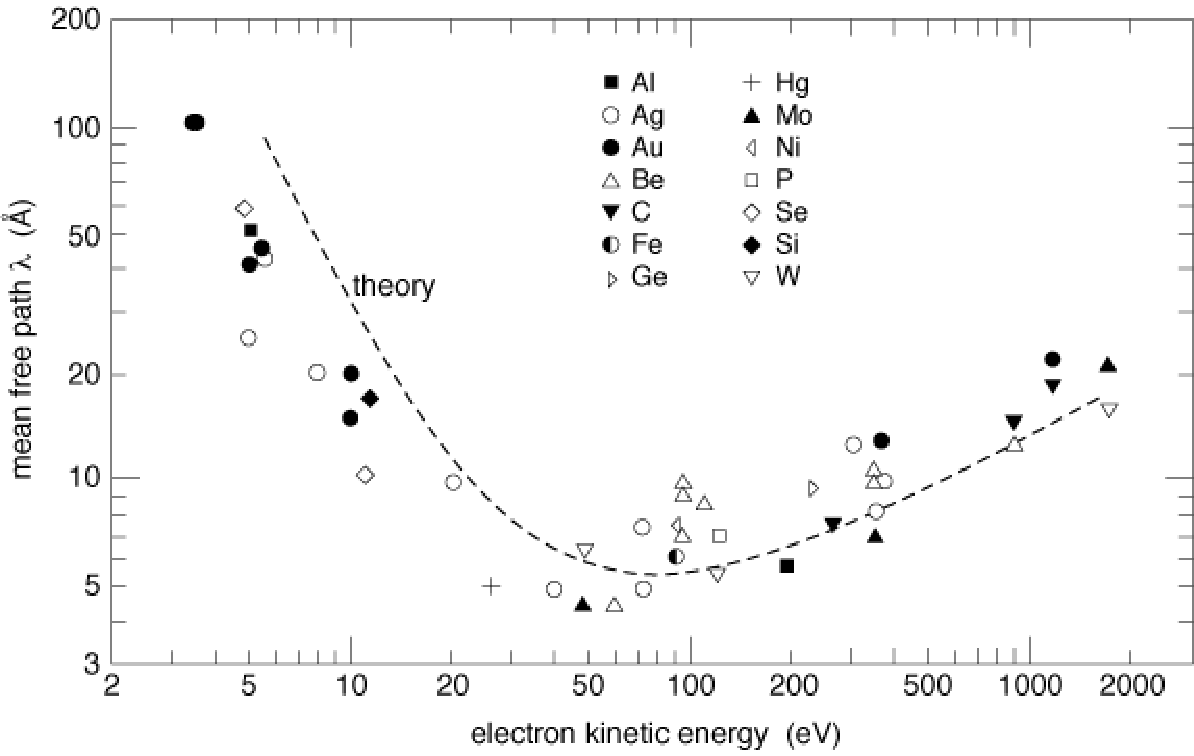
\includegraphics[width=\linewidth]{img/meanfree.pdf}

 \caption{\small Universal curve of solids \cite{zangwill}.  }
        \label{fig:uni}
\end{wrapfigure}
\FloatBarrier

\subsection{Energy Spectrum}







\clearpage
\section{Experimental Set-Up and Measurement Procedures}
\FloatBarrier
\subsection{Ultra High Vacuum (UHV)}
As the electrons used for spectroscopy easily interact with all kind of materials, it is very useful to operate in high vacuum. This is also necessary in order to reduce the rate of adsorption of molecules, which leads to disturbance of the measured spectra. (Ultra) high  vacuum (UHV) can only be achieved by a series of pumps acting within different pressure ranges. The four types used in the experiment are listed in table \ref{tab:pump}.
\begin{wraptable}{r}{0.55\textwidth}
\begin{tabular}{lr}
\toprule
pump & pressure range (Pa)\\
\midrule
\small rotary vane pump & $10^5$ - $10^{-1}$  \\ 
\small turbo molecular pump &  $10^0$  - $10^{-9}$  \\
\small ion getter pump  & $ 10^{-3}$  - $10^{-9}$  \\
\small titan sublimation pump & $10^1$  - $10^{-9}$  \\
\bottomrule
\end{tabular}
\caption{Different pumps and their pressure operating range. \cite{gop} }
\label{tab:pump}
\end{wraptable}

\subsubsection{Rotary vane pump}
The rotary vane pump is a simple mechanical pump, which consists of a cylinder connecting the vacuum cell and the outer space. In the cylinder a vane rotates and thereby shovels the gas to the outside. Springs ensure optimal contact between the vane and the cylinder walls. 



\begin{figure} 
 \centering
\subfloat[][Rotary vane pump]
{        	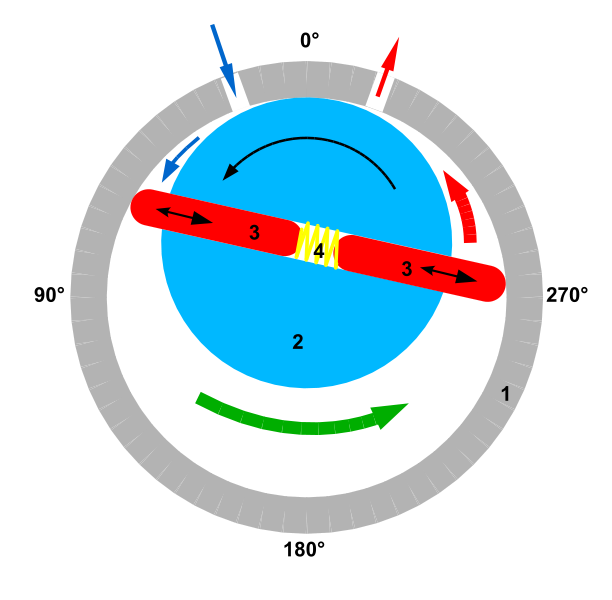
\includegraphics[width=0.45\textwidth]{img/rot.png}}
 \hfill
\subfloat[][Turbomolecular pump]
         { 	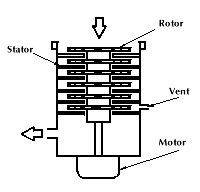
\includegraphics[width=0.45\textwidth]{img/tu.jpg}}
\caption{
\small \textbf{(a)} Rotary vane pump. 1: pump housing, 2: rotor, 3: vanes, 4: spring,  \textbf{(b)} Schematic description of a turbomolecular pump } 
	\label{fig:pump}
\end{figure}






\subsubsection{Turbomolecular pump}
The main features of a turbomolecular pump are the rotating blades (rotors), hitting the molecules very often per unit time, thereby enforcing a velocity distribution within the gas that is not isotropic, but a certain direction is preferred. Within the pump there are other static blades (stators), which act as a kind of filter to the velocity of the molecules in such a way, that molecules with the velocity, that is predominantly created by the rotors, can pass through with a higher probability. These filters act only in one-way, so that the molecules stay on the other side as long as the asymmetric velocity distribution is maintained. 






\FloatBarrier
 \bibliographystyle{unsrt}
\bibliography{bib}

\end{document}


